\chapter{BSW Modules Configuration Hints}
\label{chap:bswconfig}

This chapter provides a guideline about the expected configuration of some of the BSW Modules interacting with SrvcMgr.

%\section{BswM configuration}
%N/A
\section{Com Configuration}
\label{sec:ComConf}
The Com module must be configured to transmit the Propulsion System Active (PropSysActv) signal to the SrvcMgr module via the required port \textit{RP\_Com\_SrvcMgr\_VePSAR\_b\_PropSysActv}.

\subsection{PropSysActv Signal Configuration}
\label{sec:ComConfPropSysActv}
The Com module shall be configured with a sender-receiver interface containing the PropSysActv signal.
SrvcMgr will read this signal at runtime to determine whether RID 0x0612 can execute. The signal must be connected from the Com module to the SrvcMgr required port interface before the RTE code generation.

\section{Dcm Configuration}
\label{sec:DcmConf}
\subsection{DID 0xE0CC}
\label{sec:DcmConf0xE0CC}
The integrator should configure the DemDspDid properly for the learning table state using DID \code{0xE0CC}. 

\begin{figure}[H]
	\centering
	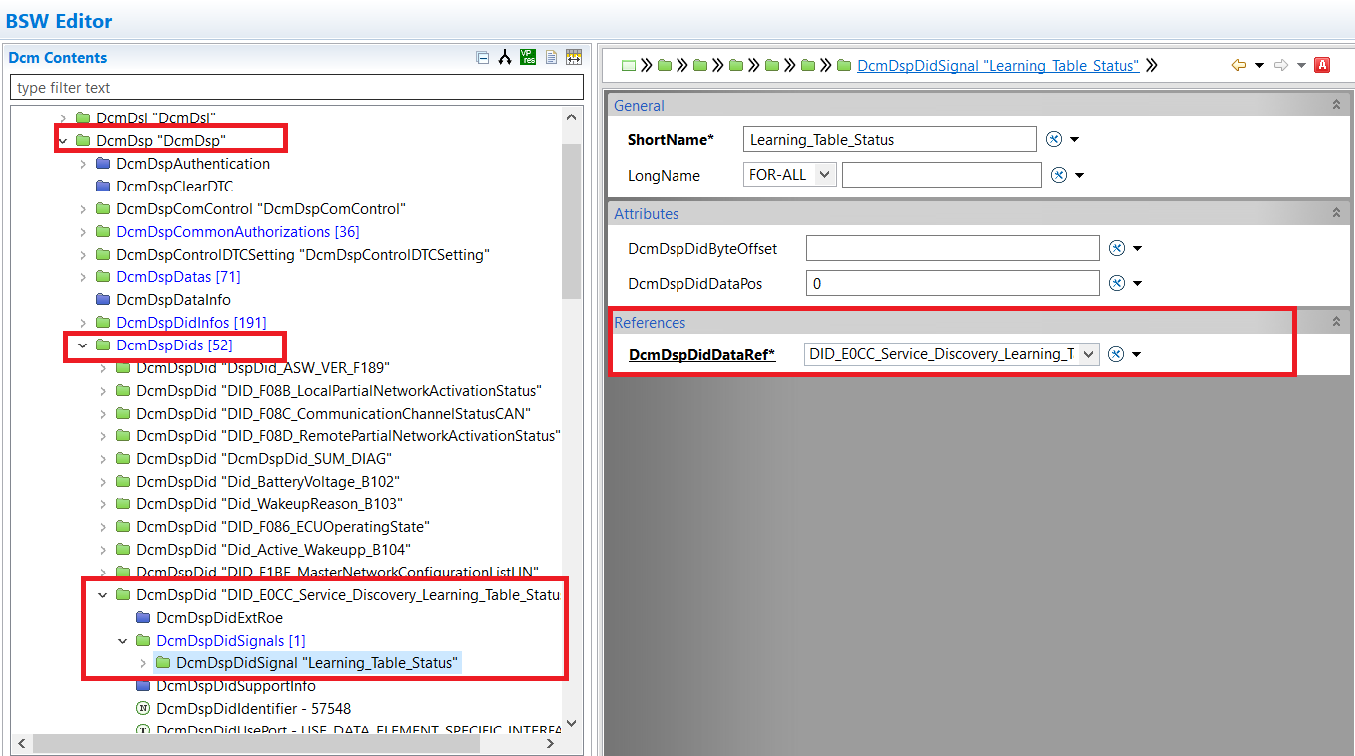
\includegraphics[scale=0.5]{images/DID_E0CC.png}
\end{figure}
\textbf{NOTE:} There should be one DemDspDidSignal configured for the DID \code{0xE0CC} since value of the learning table state is 1 byte.

\subsection{DID 0xE0CD and DID 0xE0CE}
\label{sec:DcmConf0xE0CD}
The integrator should configure the DcmDspDid as described later in order to let the SrvcMgr work properly. These two DIDs have a similar configuration as reported by SDV-6001 27.27.180.3p0.
To avoid redundancies, images reported are just for the DID 0xE0CD.
\\At the end of the configuration, the integrator should obtain something similar:
\begin{figure}[H]
	\centering
	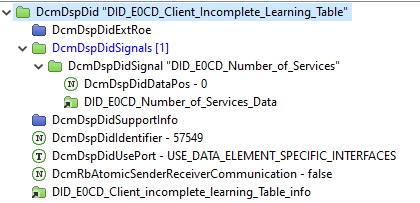
\includegraphics[scale=1]{images/DID_0xE0CD_General.png}
\end{figure}

Where the data referenced is the following: \\
\begin{figure}[H]
	\centering
	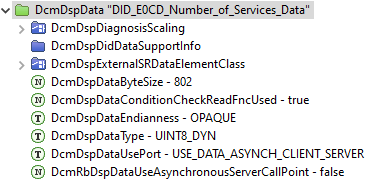
\includegraphics[scale=1]{images/DID_0xE0CD_Data.png}
\end{figure}

\subsection{RID 0x0654}
\label{sec:RID0654}
The integrator should configure the DcmDspRoutine as described to ensure that SrvcMgr works properly.
At the end of the configuration, the integrator should achieve something similar to the following:
\begin{figure}[H]
	\centering
	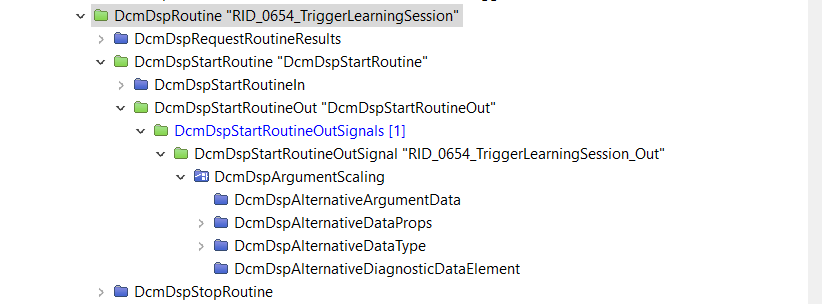
\includegraphics[scale=0.9]{images/RID_0654.png}
\end{figure}

Please pay attention to setting the parameters Position, Length, and Type as described in the SDV-6001 document.

The names of the signals are not relevant for the SrvcMgr module since it retrieves the names from the configuration.

Moreover, the integrator needs to set the name of the function in the parameter DcmRbDspRoutineUserRoutineModeRuleFnc that the DCM will call to check the Enable Conditions of the RID.
\\The definition of the function itself shall be done by the integrator.
\begin{figure}[H]
	\centering
	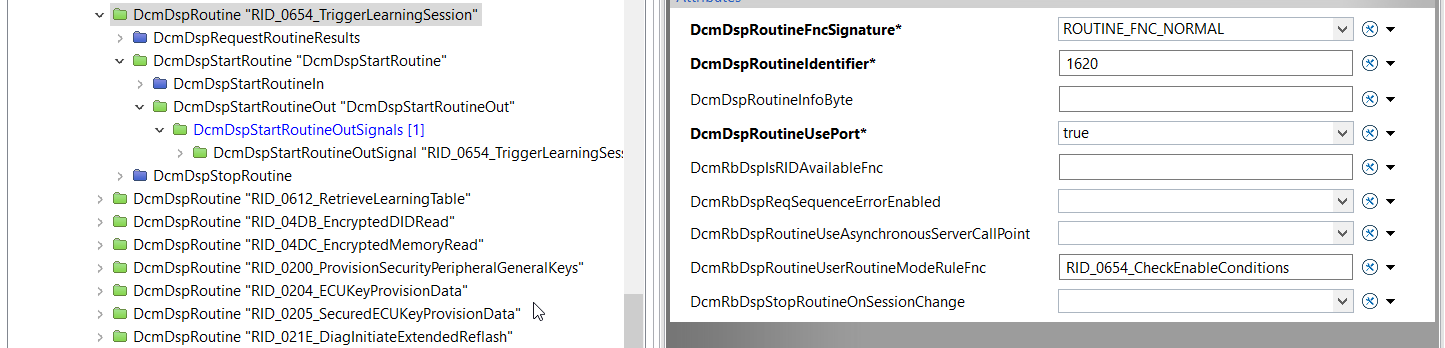
\includegraphics[scale=0.5]{images/RID_0654_CheckEnableCondition.png}
\end{figure}

Please, connect the RPort RP\_SrvcMgr\_SPM\_SdLearningStatusIndication to the SPM in order to inform SPM about Learning Session status. 

\subsection{RID 0x0612}
\label{sec:DcmConf0x0612}
The integrator should configure the DcmDspRoutine as described later in order to let the SrvcMgr works properly.
\\At the end of the configuration, the integrator should obtain something similar:
\begin{figure}[H]
	\centering
	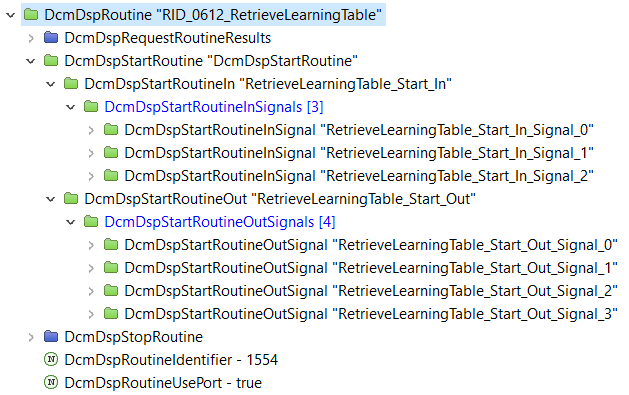
\includegraphics[scale=1]{images/RID_0x0612_General.png}
\end{figure}

The integrator shall add three DcmDspStartRoutineInSignal (one for each Control Option) following the specification in the SDV-6001 document. Please, pay attention to the fact that is necessary that the parameter DcmDspRoutineSignalPos
shall be set as following: 
\begin{itemize}
\item 0 for Control Option \#1;
\item 8 for Control Option \#2;
\item 16 for Control Option \#3;
\end{itemize}
\begin{figure}[H]
	\centering
	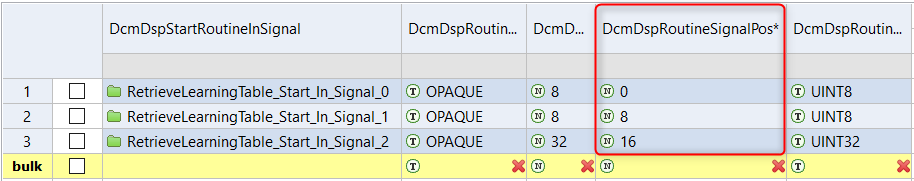
\includegraphics[scale=0.8]{images/RID_0x0612_SignalIn.png}
\end{figure}

The integrator shall add three DcmDspStartRoutineOutSignal (one for each Routine Status) following the specification in the SDV-6001 document. Please, pay attention to the fact that is necessary that the parameter DcmDspRoutineSignalPos
shall be set as following: 
\begin{itemize}
\item 0 for Routine Status \#1;
\item 8 for Routine Status \#2;
\item 24 for Routine Status \#3;
\item 56 for Routine Status \#4;

Moreover, the parameter DcmDspRoutineSignalType of Routine Status \#4 shall be set to VARIABLE\_LENGTH. 
\end{itemize}
\begin{figure}[H]
	\centering
	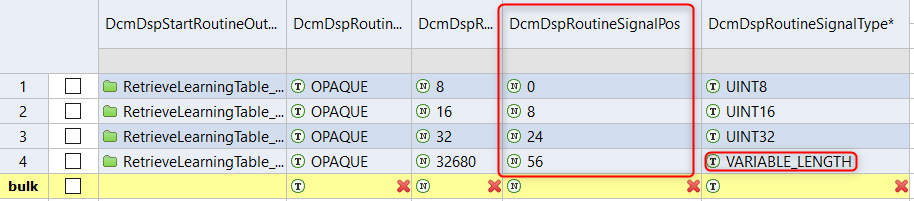
\includegraphics[scale=0.8]{images/RID_0x0612_SignalOut.png}
\end{figure}

The name of the signals are not relevant for the SrvcMgr module since it retrieve the names from the configuration.

Moreover, the integrator needs to set the name of the function in the parameter DcmRbDspRoutineUserRoutineModeRuleFnc that the DCM will call to check the Enable Conditions of the RID.
\\The definition of the function itself shall be done by the integrator.
\begin{figure}[H]
	\centering
	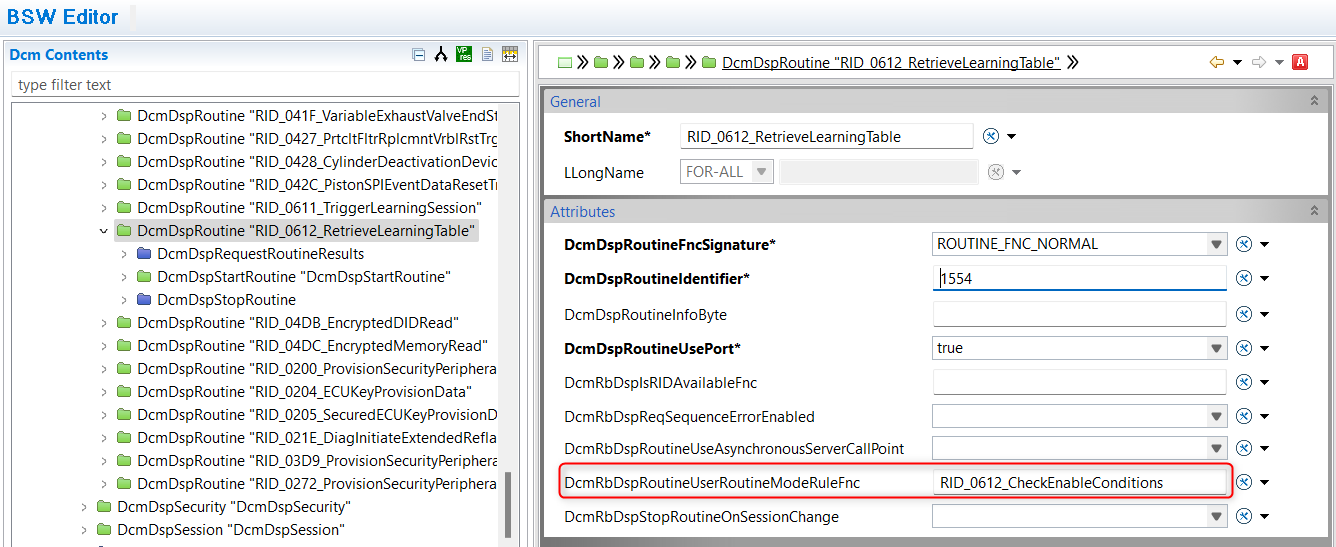
\includegraphics[scale=0.5]{images/RID_0612_CheckEnableCondition.png}
\end{figure}

\section{Dem Configuration}
\label{sec:DTCDemConf}
The DTC U19A6 46 is not managed by the Service Manager.
\\
\textbf{NOTE:}  The preconditions for the DTC U19A6 46 shall be configured by the Tier1 in the Dem module.